\section{Context}

ouldering is a form of rock climbing where climbers tackle short but challenging routes, typically lasting around 4 minutes. During this time, climbers have the freedom to choose their climbing strategies, retry as many times as needed, and aim to complete the route as quickly as possible. The ultimate goal is to reach the top of the climb in the least amount of time.

This research project is part of a larger initiative (ANR) aimed at improving bouldering performance. The focus is on developing tools for coaches to analyze bouldering performances, allowing them to provide better advice to help climbers improve.

Among these tools are: Grip Detection, Path Tracking, Performance Analysis, and more. Several models have already been developed as part of this broader effort, including a model for detecting the grips used by the climber and another for tracking the climber's path during a climb.

These models provide valuable data, but in order to fully analyze a climber's performance, it is essential to distinguish between the different phases of a bouldering event (Climbing, Observing, Brushing). By doing so, we can apply the appropriate model to each phase and gather the corresponding statistics.

This brings us to my current research project. I will be focusing on Temporal Action Segmentation (TAS), a technique that will allow us to run the grip and path analysis models at the correct timestamps. This step is crucial for gaining deeper insights into the different phases of climbing, such as observing, reading the route, and brushing the grips. By analyzing the durations, order, and impact of these phases on a climber's final performance, we can provide more precise guidance to coaches and improve training methods.

% \begin{figure}[!htbp]
\begin{figure}[H]
    \centering
    \begin{minipage}{0.24\textwidth}
        \centering
        \setlength{\fboxsep}{0pt}
        \setlength{\fboxrule}{1pt}
        \fbox{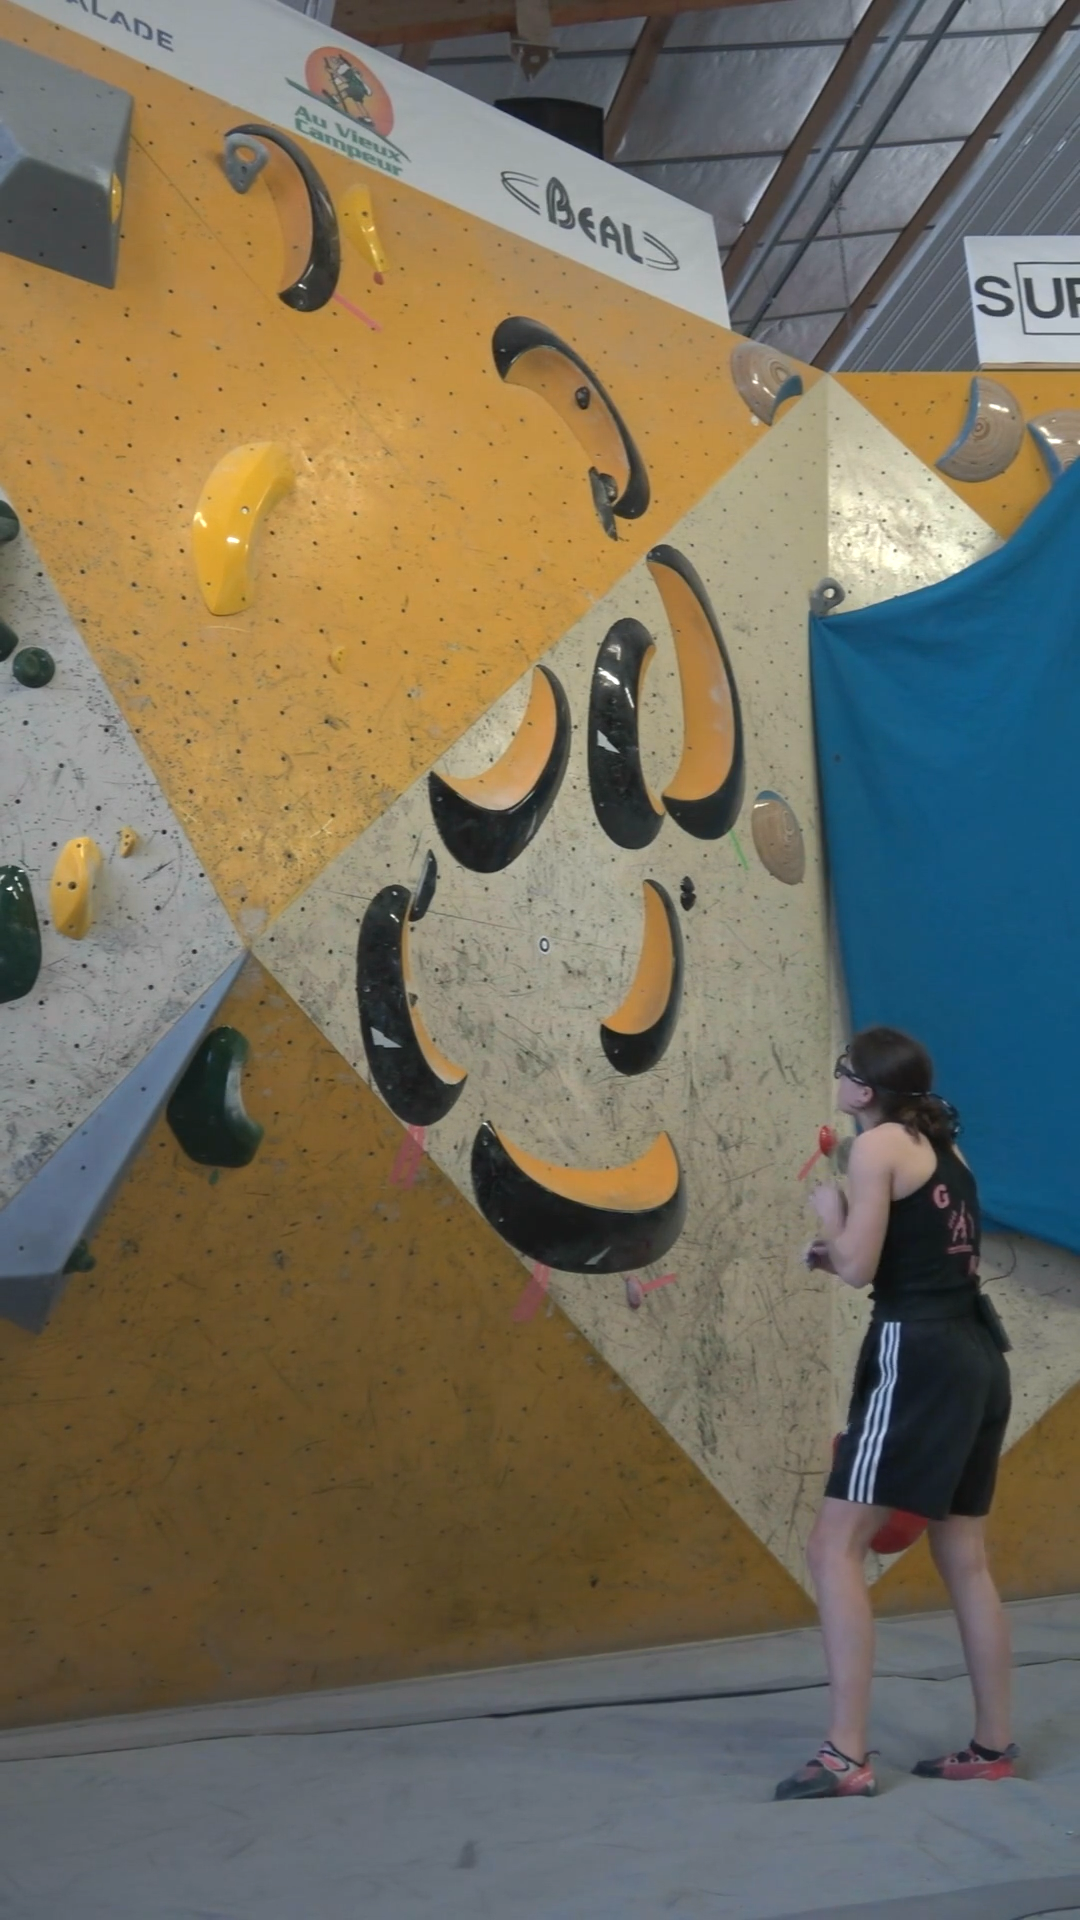
\includegraphics[width=\textwidth-2\fboxrule]{assets/images/observing.2.png}}
        \caption{Observing the block.}
        \label{fig:observing-the-block}
    \end{minipage}
    \hfill
    \begin{minipage}{0.24\textwidth}
        \centering
        \setlength{\fboxsep}{0pt}
        \setlength{\fboxrule}{1pt}
        \fbox{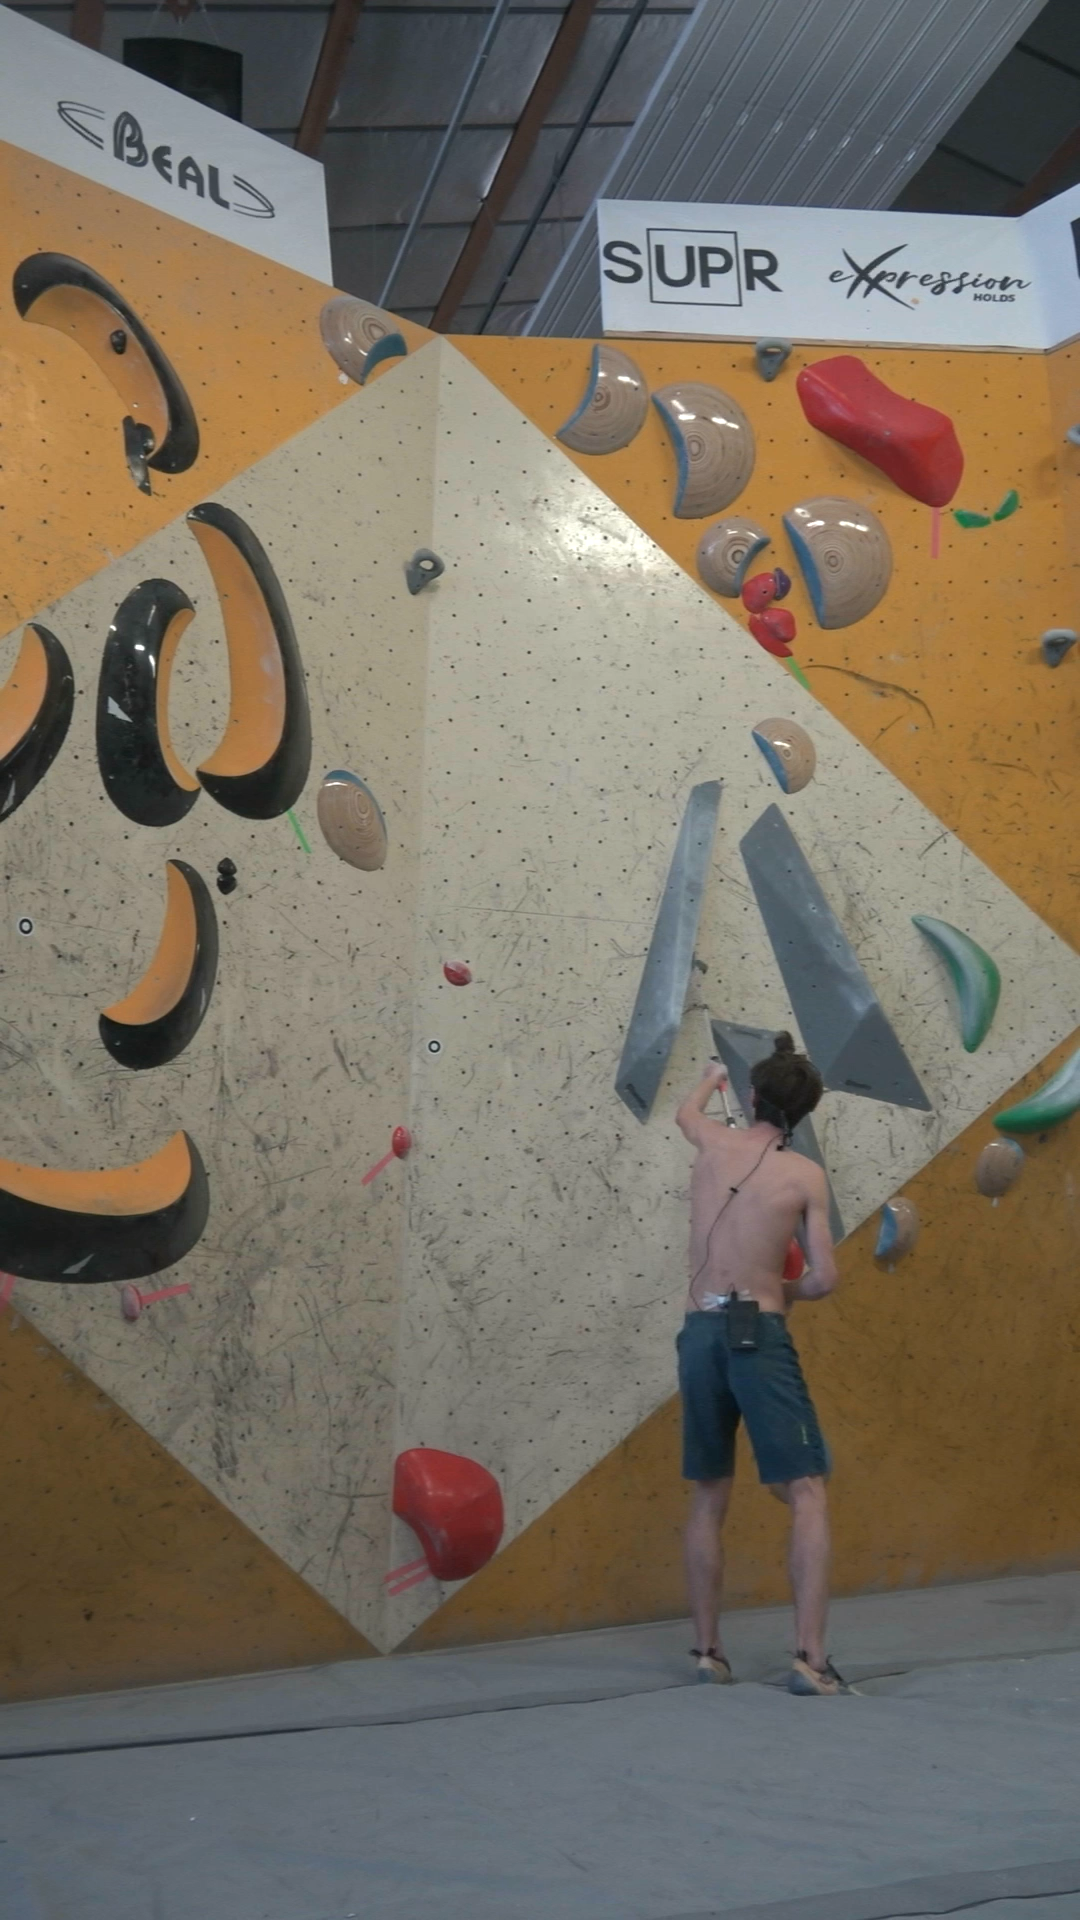
\includegraphics[width=\textwidth-2\fboxrule]{assets/images/brushing.3.png}}
        \caption{Brushing the grips.}
        \label{fig:brushing-the-grips}
    \end{minipage}
    \hfill
    \begin{minipage}{0.24\textwidth}
        \centering
        \setlength{\fboxsep}{0pt}
        \setlength{\fboxrule}{1pt}
        \fbox{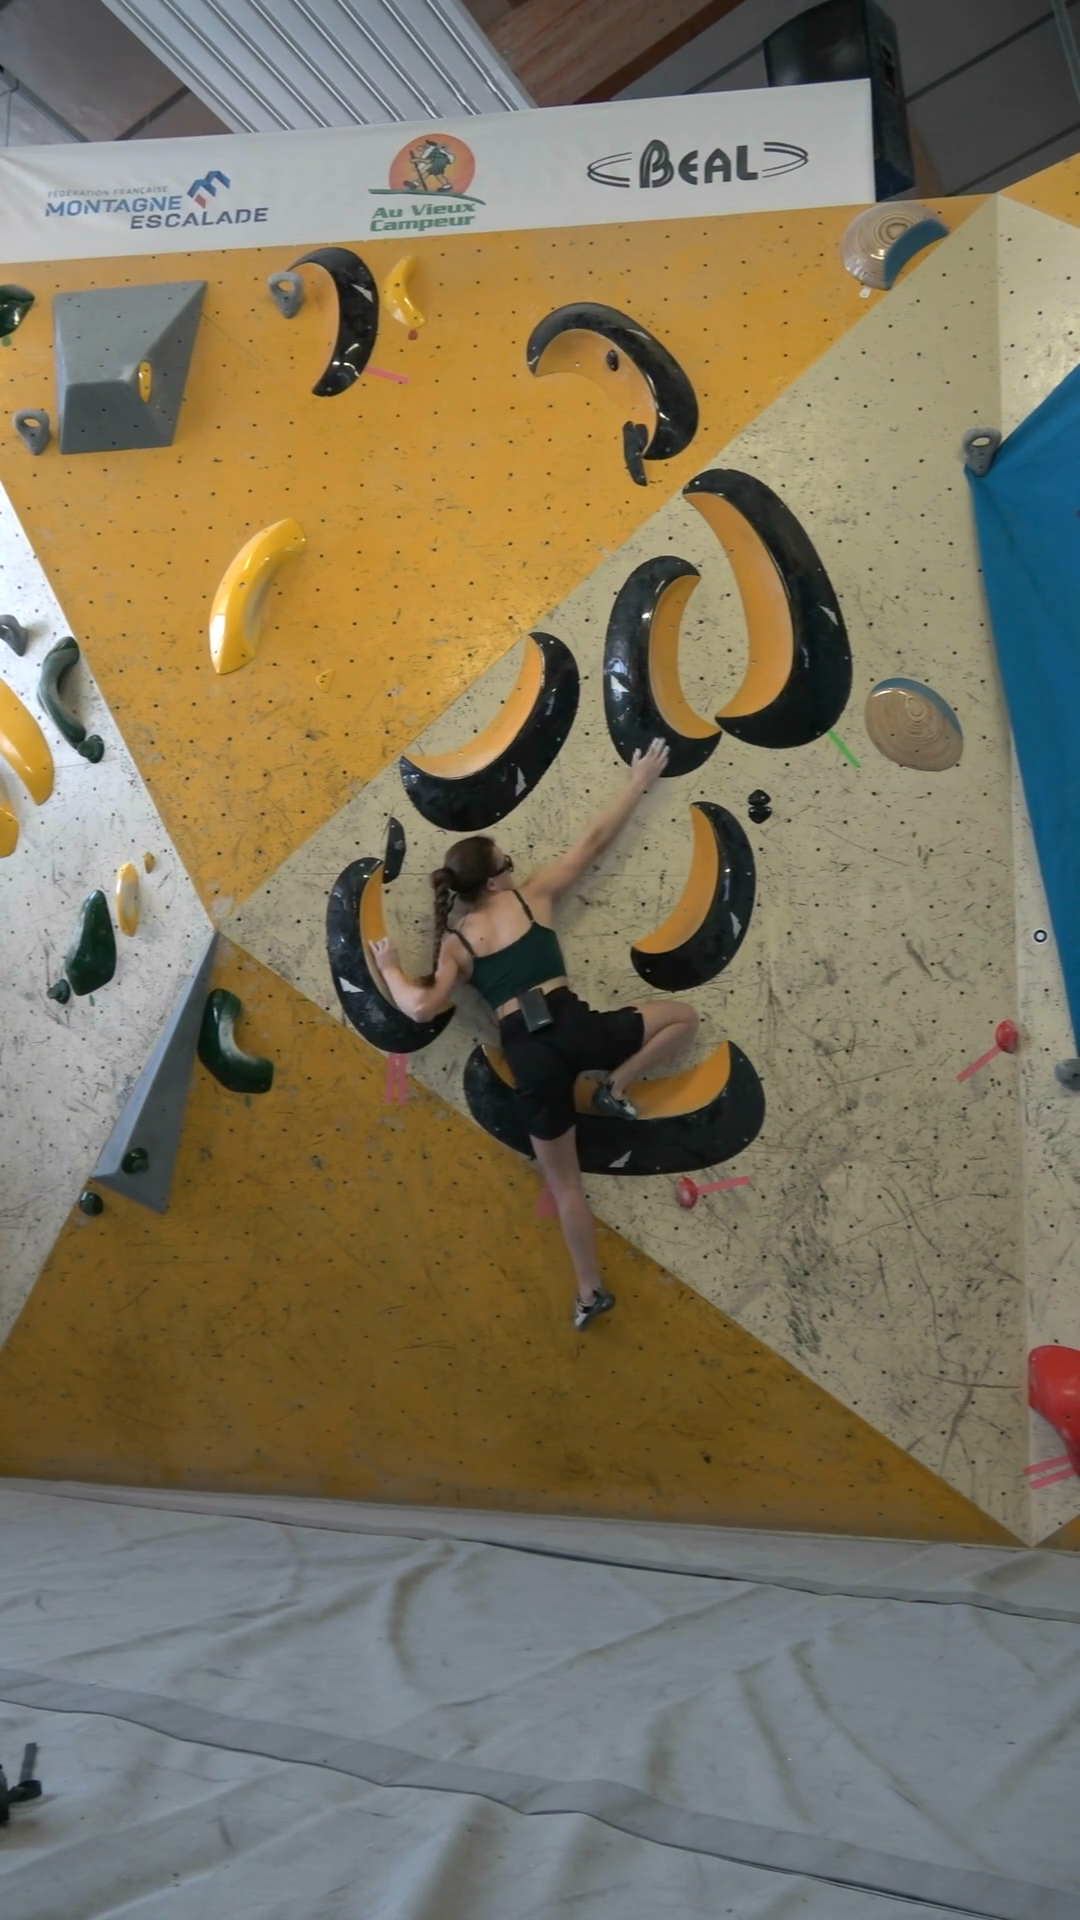
\includegraphics[width=\textwidth-2\fboxrule]{assets/images/climbing.1.png}}
        \caption{Climbing the block}
        \label{fig:climbing-the-block-1}
    \end{minipage}
    \hfill
    \begin{minipage}{0.24\textwidth}
        \centering
        \setlength{\fboxsep}{0pt}
        \setlength{\fboxrule}{1pt}
        \fbox{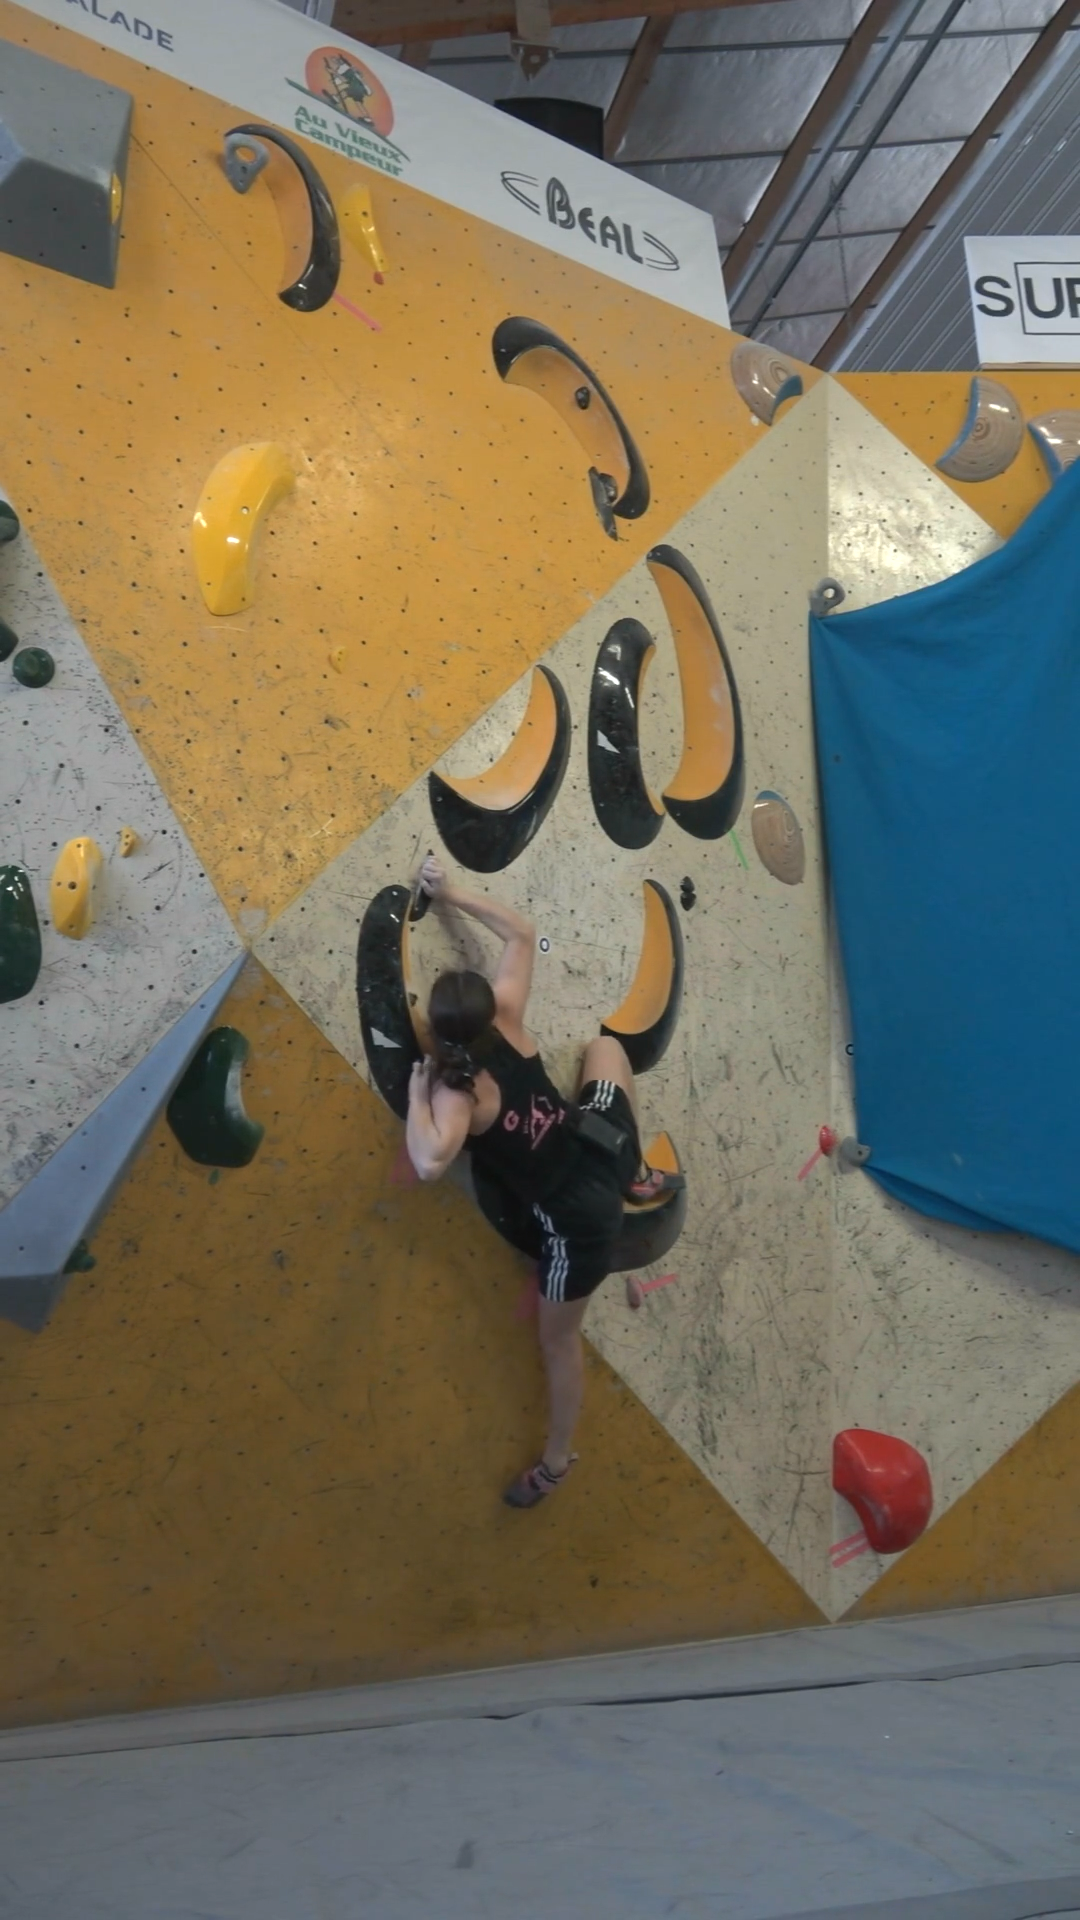
\includegraphics[width=\textwidth-2\fboxrule]{assets/images/climbing.2.png}}
        \caption{Climbing the block}
        \label{fig:climbing-the-block-2}
    \end{minipage}
\end{figure}